% Compiled using XeLaTeX
\documentclass[12pt,letterpaper]{article}
\usepackage[margin=1in]{geometry}
\usepackage{setspace}
\doublespacing
\setlength{\parindent}{0.5in}
\usepackage{indentfirst}
\usepackage{amsmath,amssymb,amsfonts}
\usepackage{algorithmic}
\usepackage{textcomp}
\usepackage{fontspec}
\usepackage{xcolor}
\usepackage{graphicx}
\usepackage{authblk}
\usepackage{microtype}
\usepackage{csquotes}
\usepackage[backend=biber,style=apa]{biblatex}
\addbibresource{rag.bib}
\let\cite\parencite
\usepackage{titlesec}
\usepackage{fancyhdr}
\usepackage{url}

% Font required by DARJ
\setmainfont{Times New Roman}

% Add the running title and page number at the top of the page
\pagestyle{fancy}
\fancyhf{}
\fancyhead[L]{\MakeUppercase{RAG for DoW Test \& Evaluation}}
\fancyhead[R]{\thepage}
\setlength{\headheight}{28pt}
\renewcommand{\headrulewidth}{0pt}

% Top Level Section Format
\titleformat{\section}
  {\bfseries\centering}
  {}
  {0pt}
  {}

% Level 2 Subsection Format
\titleformat{\subsection}
  {\bfseries\raggedright}
  {}
  {0pt}
  {}

% Level 3 Subsection Format
\titleformat{\subsubsection}
  {\bfseries\itshape\raggedright}
  {}
  {0pt}
  {}

% Title
\title{\bfseries\centering RAG for DoW Test \& Evaluation: Architecture, Security, and Automated Report Generation}
% Title and authors (authblk)
\author[1]{Michael Soltys}
\author[1]{Sam Bright}
\affil[1]{GBL Systems Corp.}
\date{\today}

\begin{document}
\maketitle

\begin{abstract}
\begin{spacing}{1.0}
This paper presents a comprehensive examination of Retrieval-Augmented Generation (RAG) as a production-deployable AI capability for Department of War (DoW) Test and Evaluation (T\&E) programs. The paper is organized around four core arguments: (1) RAG architecturally outperforms general-purpose Large Language Models (LLMs) for domain-specific T\&E tasks by grounding inference in authoritative, mission-curated knowledge bases rather than relying solely on parametric memory; (2) production DoW RAG systems require a specific, layered architecture spanning document ingestion, vector indexing, retrieval orchestration, generation, and observability, deployable across cloud impact levels IL4 through IL6; (3) operating RAG with Controlled Unclassified Information (CUI) and classified data requires a security control regime drawn from NIST SP 800-53, the DoD Risk Management Framework (RMF), CMMC, Zero Trust Architecture (ZTA) principles, and DISA impact-level guidance; and (4) few-shot prompting transforms a RAG question-answering pipeline into a structured, automated report generation capability that materially reduces analyst workload and accelerates T\&E deliverables such as Test Plans, Test Reports, and Interim Fielding Assessments. Together these arguments establish the theoretical and practical foundation for a full-lifecycle RAG deployment within a DoW T\&E enterprise. We ground the discussion in a case study of a production RAG system the authors deployed on AWS GovCloud for a Navy warfare center, providing concrete evidence of the layered architecture in operational use.
\end{spacing}
\end{abstract}

% Keywords (Chicago style paragraph)
\vspace{1em}
\noindent\textbf{Keywords:}
Retrieval-Augmented Generation, Large Language Models, Test and Evaluation, Few-Shot Prompting, DoW Cloud Security

\section{Introduction}

Large Language Models have emerged as transformative tools across government and industry, yet their application to Department of War Test and Evaluation programs presents acute challenges. LLMs store knowledge in fixed model weights trained on a static corpus; once training ends, the model cannot access updated information without retraining \cite{lewis2020,gao2023}. For T\&E environments, this creates three critical failure modes: knowledge staleness, as test procedures, system specifications, and MIL-STDs evolve continuously; hallucination under domain sparsity, where models generate plausible but factually incorrect outputs in safety-critical reporting contexts; and non-traceability, where outputs cannot be traced to specific authoritative sources, violating DoW documentation standards that require cited, auditable evidence.

Retrieval-Augmented Generation, first formally introduced by \textcite{lewis2020} at Facebook AI Research, addresses these limitations by combining pre-trained parametric memory (the LLM) with non-parametric memory (a dense vector index of documents) accessed through a pre-trained neural retriever. The original formulation proposed two architectures: RAG-Sequence, where the same retrieved document conditions the entire generated sequence, and RAG-Token, where different documents can inform different output tokens. Both achieved state-of-the-art results on open-domain question answering, outperforming both parametric-only and extractive retrieval-based approaches \cite{lewis2020}. RAG has since become the dominant approach for knowledge-grounding LLMs in enterprise and government contexts, enabling dynamic knowledge updates without retraining, source attribution that satisfies DoW traceability requirements, cost-efficient knowledge base maintenance, substantial hallucination reduction, and regulatory alignment through classification-aware metadata \cite{aws2025,ibm2025}.

The DoW has signaled that RAG is not merely a research interest but an operational mandate. In January 2026, the Department of the Navy formally designated GenAI.mil---which provides RAG for sourcing answers from uploaded documents, secure web grounding, and deep research capabilities---as the mandated CUI and IL5 generative AI platform for all DON users, directing all organizations and commands to transition no later than April 30, 2026 \cite{don_genai2026}. This enterprise-level mandate, issued jointly by the Assistant Secretary of the Navy for Research, Development, and Acquisition and the DON Chief Information Officer, confirms that RAG-enabled AI is now an institutional requirement rather than an optional capability.

This paper presents a comprehensive examination of RAG as a production-deployable capability for DoW T\&E programs. We argue that RAG architecturally outperforms general-purpose LLMs for domain-specific T\&E tasks, that production deployment requires a specific layered architecture deployable across cloud impact levels IL4 through IL6, that operating with CUI and classified data demands a rigorous security control regime, and that few-shot prompting transforms RAG from a question-answering tool into a structured automated report generation capability. We illustrate these arguments with a case study of a production deployment the authors built on AWS GovCloud for a Navy warfare center. Together these arguments establish the foundation for full-lifecycle RAG deployment within a DoW T\&E enterprise.

\paragraph{A note on terminology and applicability.}
The discussion below uses U.S.~Department of War (DoW) terminology because the case study and most cited policy artifacts are American---``IL4 through IL6'' for tiered cloud impact levels, ``Controlled Unclassified Information (CUI)'' for the standard sensitive-but-unclassified category, ``NIPRNet'' and ``SIPRNet'' for the unclassified and secret government networks, ``Authorization to Operate (ATO)'' for system accreditation, ``CMMC'' for supplier cyber-maturity certification, and ``CDAO'' for the central defence AI office. Equivalent constructs exist in most allied defence establishments and in many regulated civilian sectors (health, finance, critical infrastructure): the architectural, security, and report-automation patterns we describe transfer with the labels swapped. Where a DoW-specific term first appears, we have tried to expand the acronym and (where useful) note the generic concept it instantiates so readers in other ministries, agencies, or industries can map the discussion onto their own equivalents.

\section{How RAG works and why it outperforms general-purpose LLMs for T\&E}

\subsection{Fundamental Limitations of Parametric-Only LLMs}

Fine-tuning as an alternative to RAG incurs high retraining compute costs, degrades performance on tasks outside the fine-tuned domain, and still cannot access information created after training \cite{stackoverflow2023,f22labs2024}. In T\&E contexts, where test procedures, system specifications, and military standards evolve continuously, a static LLM cannot track updates without costly fine-tuning cycles. When a model lacks sufficient domain-specific training data, it generates plausible-sounding but factually incorrect outputs---a critical risk in safety-critical T\&E reporting.

\subsection{The RAG Paradigm: Architecture and Mechanism}

The core RAG pipeline consists of four stages (Figure~\ref{fig:rag-pipeline}). First, document ingestion and preprocessing: raw T\&E artifacts---test plans, test reports, specifications, CONOPS, MIL-STDs---are parsed, normalized, and segmented into chunks. Second, embedding and indexing: each chunk is encoded into a dense vector representation by an embedding model and stored in a vector database alongside metadata including document title, classification marking, date, and system identifier. The key insight is that embeddings encode semantic meaning, not keywords: sentences with entirely different words but similar meaning (e.g., ``the dog chased the ball'' and ``a puppy ran after a sphere'') are mapped to nearby points in vector space, enabling semantic retrieval that keyword search cannot achieve. Third, query-time retrieval: when a user submits a query, the query is embedded using the same embedding model, and cosine similarity or approximate nearest-neighbor search retrieves the top-$k$ most relevant chunks from the vector store. Fourth, augmented generation: retrieved chunks are injected into the LLM's context window as grounding evidence, and the LLM synthesizes a response anchored to that evidence rather than relying solely on parametric memory \cite{aws2025,ibm2025}.

\begin{figure}[htbp]
\centering
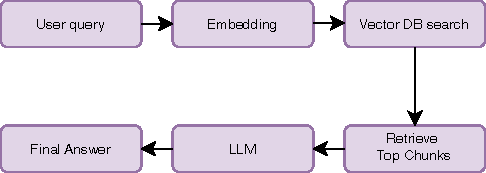
\includegraphics[width=\textwidth]{figures/rag-pipeline.pdf}
\caption{Core RAG pipeline showing the query-time retrieval flow (top) and document ingestion path (bottom). The embedding model creates dense vector representations that enable semantic matching between queries and document chunks.}
\label{fig:rag-pipeline}
\end{figure}

Chunking strategy critically affects retrieval quality. Chunks that are too small fragment context and lose coherence; chunks that are too large waste the LLM's context window and dilute focus. \textcite{wang2024rag} conducted systematic experiments comparing chunk sizes of 128, 256, 512, 1024, and 2048 tokens, finding that 512-token chunks achieved the highest average faithfulness score (97.59\%) while 256-token chunks achieved the highest relevancy (97.78\%), with both substantially outperforming the 2048-token baseline (80.37\% faithfulness, 91.11\% relevancy). Among chunking techniques, the sliding window approach---which uses overlapping chunks to prevent boundary information loss---outperformed both original chunking and the small-to-big method, achieving 97.41\% faithfulness and 96.85\% relevancy \cite{wang2024rag}. Semantic-boundary chunking at paragraph or section boundaries is preferred over fixed-token chunking for structured T\&E documents.

RAG implementations have evolved through several generations (Figure~\ref{fig:naive-vs-advanced}). Naive RAG performs simple single-pass retrieve-then-generate operations but is prone to low-precision retrieval and context misalignment. Advanced RAG incorporates pre-retrieval query expansion, re-ranking, post-retrieval compression, and relevance filtering to improve chunk quality \cite{gao2023,promptingguide2024}. Re-ranking---using deep language models to re-score retrieved chunks by relevance---dramatically improves retrieval precision. On the MS MARCO passage ranking benchmark, DLM-based re-rankers such as RankLLaMA achieved MRR@1 scores of 22.08 compared to 6.52 for BM25 alone, representing a 3.4$\times$ improvement, while Hit Rate@10 rose from 24.63 to 54.53 \cite{wang2024rag}. Modular RAG introduces composable pipeline nodes including specialized retrievers, memory modules, adaptive retrieval triggers, and iterative retrieval for complex multi-hop queries. Agentic RAG represents the emerging frontier, where an LLM orchestrator autonomously decides when retrieval is needed, formulates sub-queries, and integrates multiple retrieval rounds---a pattern already appearing in Chief Digital and Artificial Intelligence Office (CDAO) AI Rapid Capabilities Cell pilots \cite{gdit2024}.

\begin{figure}[htbp]
\centering
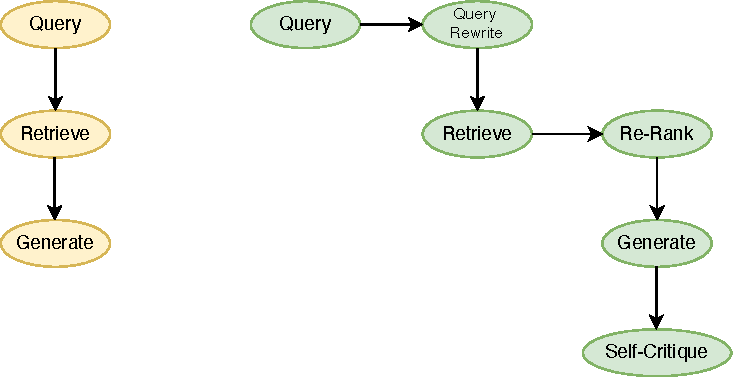
\includegraphics[width=0.85\textwidth]{figures/naive-vs-advanced-rag.pdf}
\caption{Naive RAG versus Advanced RAG. Naive RAG performs a single retrieve-then-generate pass. Advanced RAG adds query rewriting, re-ranking, and self-critique stages that substantially improve accuracy for production deployments.}
\label{fig:naive-vs-advanced}
\end{figure}

Three common failure modes must be addressed in production RAG systems. First, retrieval misses relevant chunks---mitigated through better chunking strategies, query rewriting, higher $k$ values, and re-ranking. Second, the model ignores good context---mitigated through explicit prompt instructions such as ``Answer ONLY from provided context; if the information is not there, say so.'' Third, hallucinations persist despite retrieved context---mitigated by requiring the model to quote source passages before generating answers, forcing citation-grounded output.

\subsection{Why RAG Dominates Fine-Tuning for T\&E Domains}

RAG offers decisive advantages over fine-tuning for T\&E applications. RAG knowledge bases can be updated asynchronously---new test results, updated specifications---without retraining the LLM, whereas fine-tuned models require full retraining cycles \cite{stackoverflow2023,ibm2025}. RAG returns the retrieved document chunks alongside the generated answer, enabling analysts to verify outputs against primary sources and satisfying DoW documentation traceability requirements \cite{aws2025}. Updating a vector index is orders of magnitude cheaper than re-running a fine-tuning run on GPU clusters \cite{f22labs2024}. Studies show accuracy and usefulness improvements of 107--177\% on domain question-answering tasks when RAG is applied versus zero-shot LLM baselines \cite{arxiv2511}. Retrieved documents carry classification markings and provenance metadata, enabling access-controlled generation consistent with CUI and SAP handling requirements.

The simplest mental model: RAG combines a librarian with a language model. The librarian searches the knowledge base and hands over relevant pages; the model reads those pages and writes the answer. Most RAG failures trace to one of two causes: the wrong documents were retrieved, or the model failed to use the documents it was given. This framing clarifies that RAG quality depends as much on retrieval engineering as on the generative model.

RAG is not universally appropriate. When the entire knowledge base fits within a single LLM context window, direct context injection (``stuffing'') is simpler and avoids retrieval latency. When the task requires holistic reasoning over an entire corpus rather than targeted retrieval, RAG's chunk-based approach may fragment necessary context. When latency is critical and retrieval adds unacceptable delay, or when the underlying data changes every few seconds faster than embeddings can be refreshed, alternative architectures may be preferred. For deeply internalized, static domain knowledge, fine-tuning remains appropriate. T\&E applications, however, are characterized by large, evolving document corpora and strict traceability requirements---precisely the conditions where RAG excels.

\subsection{T\&E-Specific Advantages}

T\&E knowledge bases include MIL-STDs, test procedures, previous test reports, systems engineering documents, specification trees, and operator manuals---all ideal RAG corpus material. RAG can retrieve and synthesize across hundreds of T\&E artifacts simultaneously, a task no single analyst can perform manually at scale. The knowledge base ingestion pipeline can be triggered on a schedule to capture new test data as it is generated, keeping the system current with ongoing test programs. Because retrieved context is logged alongside the generated answer, each output can be reproduced and audited---essential for test record integrity.

\subsection{Quantitative Performance Benchmarks}

The RAGAS framework evaluates RAG systems on context relevance, answer faithfulness, and answer relevance, outperforming hand-written heuristic baselines \cite{ares2024}. The BEIR benchmark suite demonstrates that RAG-augmented models consistently outperform standalone LLMs on knowledge-intensive tasks across diverse domains. Enterprise systematic literature review findings indicate that 80.5\% of enterprise RAG implementations use standard retrieval frameworks such as FAISS and Elasticsearch, GPT-based models dominate at 63.6\%, and domain-specific corpora markedly outperform generic public corpora \cite{mdpi2025}. Readers seeking a more comprehensive treatment of the broader RAG evaluation landscape are referred to the recent PRISMA-aligned systematic review of \textcite{brown2025}, which catalogues the field's evolution from DPR-based baselines toward modular, policy-driven architectures with hybrid retrieval and uncertainty-aware control, and to \textcite{yu2025rag}, who propose a unified evaluation framework distinguishing retrieval, generation, and end-to-end metrics.

\section{Architecture and technology stack for production DoW RAG deployment}

A production DoW RAG system is not a single application but a multi-layer data and AI platform. Treating it as an ad hoc chatbot feature is the primary cause of failed deployments \cite{devcommunity2025}. Recent surveys of the RAG stack synthesize academic and industrial deployment experience into a unified taxonomy with explicit attention to trust, alignment, and domain adaptation \cite{wampler2026}, mirroring the layered, policy-driven approach we adopt below. The architecture comprises five production layers.

\subsection{Layer 1: Document Ingestion and Preprocessing}

Source connectors interface with SharePoint on NIPRNet and SIPRNet (the U.S.~unclassified and secret government networks; analogous segregated network tiers exist in other defence establishments), SIPR file shares, PDFs, Word documents, technical data packages, and structured databases. Content extraction employs Optical Character Recognition (OCR) for scanned documents, table extraction, and image captioning, with normalization to plain text or structured JSON. Metadata enrichment captures classification marking, originating organization, system program, document type, version, and date as filterable fields. Deduplication and version control detect superseded documents to prevent stale context injection.

\subsection{Layer 2: Embedding and Indexing}

Chunking strategy is critical: semantic-boundary chunking at paragraph and section boundaries is preferred over fixed-token chunking, with typical chunk sizes of 256--1024 tokens depending on document structure \cite{ijonis2026}. For cloud and NIPRNet environments, embedding models such as OpenAI text-embedding-3-large and Google text-embedding-004 are available on GenAI.mil. For air-gapped and SIPRNet environments, open-source models such as BGE-M3, multilingual-e5-large, or Nomic Embed can be deployed on self-hosted GPU nodes.

Vector databases suitable for IL5/IL6 environments include Milvus, Weaviate, Qdrant, and pgvector. A systematic comparison of five open-source vector databases against four key criteria---multiple index types, billion-scale vector support, hybrid search, and cloud-native deployment---found that Milvus was the only database satisfying all four criteria, making it the most comprehensive solution for enterprise RAG deployments \cite{wang2024rag,gigaspaces2025,zenml2025}. Hybrid search combining dense vector search with sparse BM25 keyword search (Figure~\ref{fig:hybrid-search}) consistently outperforms either method alone on T\&E terminology-heavy corpora. Pure vector search excels at semantic matching but misses exact terminology; BM25 keyword search captures precise terms but lacks semantic understanding. Systematic experiments demonstrate that hybrid search, computed as $S_h = \alpha \cdot S_s + S_d$ where $S_s$ and $S_d$ are normalized sparse and dense retrieval scores respectively, achieves optimal performance at $\alpha = 0.3$, yielding mAP of 47.14 and nDCG@10 of 72.50 on TREC DL19---substantially outperforming either BM25 (mAP 30.13) or dense retrieval alone \cite{wang2024rag}. This makes hybrid search essential for mission-critical RAG deployments where T\&E-specific terminology such as MIL-STD designators, system nomenclature, and test procedure identifiers must be matched exactly.

\begin{figure}[htbp]
\centering
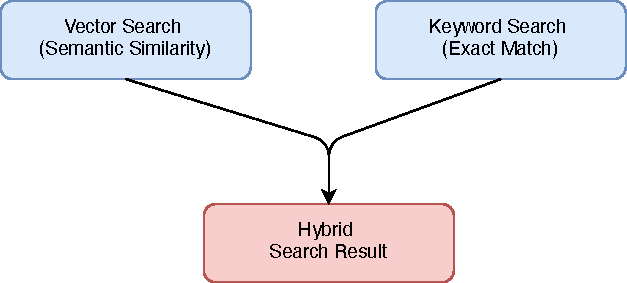
\includegraphics[width=0.7\textwidth]{figures/hybrid-search.pdf}
\caption{Hybrid search architecture combining dense vector search (semantic similarity) with sparse BM25 keyword search (exact match) for improved retrieval quality.}
\label{fig:hybrid-search}
\end{figure}

\subsection{Layer 3: Retrieval Orchestration}

A production retrieval orchestration layer implements multiple processing stages identified by \textcite{wang2024rag} as critical to RAG performance: query classification (determining whether retrieval is necessary), retrieval itself, reranking, document repacking, and summarization. Query analysis and expansion techniques include query rewriting, hypothetical document expansion (HyDE)---which generates pseudo-documents from the query and retrieves based on their embeddings---and multi-query generation to improve recall. \textcite{wang2024rag} found that combining HyDE with hybrid search achieved the best retrieval performance across benchmarks. Cross-encoder re-rankers improve precision post-retrieval, with the ``sides'' repacking method---placing the most relevant documents at both the beginning and end of the context window---achieving optimal generation performance. Metadata filtering based on access controls ensures users only retrieve documents at or below their classification and clearance level. Retrieved chunks are deduplicated, ordered by relevance, and formatted into a structured context window prompt.

\subsection{Layer 4: LLM Generation}

Model selection varies by classification level. At IL4 on NIPRNet, options include GPT-4o via Azure Government and Gemini for Government on GenAI.mil; Anthropic Claude was previously available under a DoD contract but is no longer authorized following the supply chain risk designation discussed below. At IL5 for sensitive CUI, Ask Sage on Azure Government IL5 provides dedicated instances with FedRAMP (Federal Risk and Authorization Management Program) High provisional authorization. At IL6 on SIPRNet, dedicated cloud enclaves on SIPRNet-connected infrastructure with U.S.-citizen-only personnel are required \cite{asksage2025,grsee2025}.

Prompt engineering specifies output format, citation requirements, classification handling instructions, and role definition. Few-shot examples demonstrating the target report format condition the model for structured output generation.

\subsection{Layer 5: Observability, CI/CD, and Governance}

Every query, retrieved chunk set, and generated response is logged to an immutable audit trail, mandatory for Authorization to Operate (ATO) and Security Technical Implementation Guide (STIG) compliance \cite{cdao_rmf2024}. Monitoring tracks retrieval quality metrics (nDCG, Hit Rate), generation quality metrics (faithfulness, relevance), latency, and cost. AI CI/CD encompasses version-controlled prompt templates, chunking logic, embedding models, and re-ranker configurations, with regression tests on representative T\&E queries before any pipeline update. Human-in-the-loop review is mandatory: all generated T\&E deliverables are flagged for analyst review before distribution.

\subsection{DoW-Specific Deployment Topology}

The Joint Warfighting Cloud Capability (JWCC), the DoW's enterprise multi-vendor cloud contracting vehicle, provides four enterprise cloud on-ramps---AWS, Microsoft Azure, Google Cloud, and Oracle---enabling RAG infrastructure deployment at IL2 through IL6 (DoD impact levels covering unclassified through SECRET workloads; analogous tiered government cloud accreditation regimes exist in the UK, Australia, Canada, and the EU) \cite{defensescoop2024}. CDAO AI Rapid Capabilities Cell sandboxes, launched in January 2025, provide cloud-hosted development and test environments at multiple impact levels for rapid prototyping.

Reference deployment architectures span multiple classification levels. NIPRNet at IL4 employs multi-tenant cloud RAG with Common Access Card (CAC) authenticated API gateway, Azure AD/Entra integration, and Federal Information Processing Standards (FIPS) 140-2 encryption. NIPRNet sensitive at IL5 requires a dedicated, physically isolated cloud enclave with U.S.-citizen personnel and 421+ NIST 800-53 controls. SIPRNet at IL6 requires SECRET enclaves connected to SIPRNet with active SECRET clearances, TEMPEST-shielded data centers, and disconnected-from-internet inference nodes. Tactical and denied, degraded, intermittent, or limited (DDIL) edge environments can leverage containerized RAG stacks deployable on forward operating bases, naval vessels, or disconnected operational environments \cite{asksage_dib2025}.

\subsection{Real-World DoW RAG Deployments}

GenAI.mil, launched in December 2025, provides Google Gemini with multimodal RAG and web-grounded search to 3 million DoW employees, built on Google Cloud with Anthropic, OpenAI, and xAI contracts each valued up to \$200 million at the time of award \cite{defensescoop_dec2025}; the Anthropic component was subsequently removed following the February--March 2026 supply chain risk designation discussed below. Multiple service-specific generative AI platforms have been developed and fielded on NIPRNet at IL4 with CAC authentication, with some reaching over 100,000 users within three months of launch \cite{vanroo2025}. Army, Combatant Command, and CDAO enterprise platforms each incorporate RAG at varying classification levels, demonstrating broad adoption across the DoW \cite{vanroo2025,asksage2025}.

\subsection{Orchestration Frameworks}

LangChain provides modular pipeline construction for chaining retrieval, re-ranking, and generation steps, with integrations across all major vector databases and LLM APIs. LlamaIndex is optimized for performant retrieval with strong support for structured document indexing, multi-document routing, and sub-question decomposition \cite{paragon2024}. Haystack, originally developed by deepset, offers a component-based pipeline architecture in which retrievers, embedders, rankers, and generators are composed as connected nodes, with first-class support for hybrid retrieval, prompt templating, and pluggable LLM backends---making it well suited to vendor-agnostic designs that must tolerate inference-endpoint substitution. All three frameworks support FIPS-compliant configurations and air-gapped deployment when combined with self-hosted models.

\section{Security controls for RAG systems handling CUI and classified data}

\subsection{Regulatory and Policy Framework}

DoD Instruction 8510.01 mandates the Risk Management Framework (RMF; the U.S.\ federal IT-accreditation regime built on NIST SP 800-53, broadly comparable to ISO/IEC 27001-based frameworks used elsewhere) for all DoW IT; AI systems including RAG pipelines are subject to full RMF authorization before operational deployment \cite{cdao_rmf2024}. NIST SP 800-53 Rev 5 provides the authoritative control catalog, requiring RAG systems to implement controls from Access Control, Audit and Accountability, System and Communications Protection, System and Information Integrity, and Risk Assessment families. NIST SP 800-171 Rev 3 and Cybersecurity Maturity Model Certification (CMMC) Level 2--3 apply to contractors processing CUI; as of November 2025, CMMC is in effect for DoW contracts, and RAG systems storing CUI must meet CMMC Level 2 minimum \cite{wiley2025}.

The NIST AI Risk Management Framework 1.0 with its GOVERN, MAP, MEASURE, and MANAGE functions, along with the Generative AI Profile (NIST AI 600-1), provides voluntary but strongly recommended guidance; CDAO's Responsible AI Toolkit is built on these frameworks \cite{nist2025}. The DoD Zero Trust Strategy and Execution Roadmap specifies 152 ZT activities across five phases; RAG systems must implement identity, device, network, application, and data pillars \cite{dod_zt2026}. Executive Orders 13556 and 13526 govern marking, handling, and transmission rules directly applicable to RAG knowledge base content.

\subsection{Data Security Controls for the RAG Knowledge Base}

\subsubsection{Classification-Aware Ingestion.}

Every document ingested must have its classification marking parsed and stored as a vector metadata field. Automated classification recognition using natural language processing (NLP) classifiers trained on DoW marking conventions detects and enforces markings, rejecting malformed or unclassified documents submitted to classified stores. Separate vector indexes by classification level---UNCLASSIFIED, CUI, SECRET, and TOP SECRET---must reside in logically or physically isolated index namespaces.

\subsubsection{Access Control and Least Privilege.}

Attribute-Based Access Control (ABAC) enforces query-time metadata filters ensuring users only retrieve chunks at or below their clearance and need-to-know; queries from IL4-cleared users cannot traverse IL6 vector indexes. All DoW RAG endpoints must be gated by CAC or Personal Identity Verification (PIV) authentication. Role-Based Access Control (RBAC) provides differentiated permissions for query, ingest, delete, and model configuration operations.

\subsubsection{Encryption Requirements.}

Data at rest requires AES-256 encryption on all vector database storage volumes with FIPS 140-2/140-3 validated cryptographic modules. Data in transit requires TLS 1.2 minimum with TLS 1.3 preferred for all API calls between RAG components, and mutual TLS for service-to-service communication. Embedding vector confidentiality must be maintained through dedicated inference nodes and secure enclaves, as embedding models can leak information via vector similarity attacks.

\subsection{AI-Specific Threats and Mitigations}

Prompt injection and indirect prompt injection occur when adversarial input in retrieved documents instructs the LLM to override system prompt instructions. Mitigations include input sanitization at ingestion, prompt shields, and output validation to detect instruction-following anomalies \cite{microsoft2026}.

Knowledge base poisoning represents a particularly acute threat. \textcite{zou2025} demonstrated with PoisonedRAG that injecting just five malicious texts into a knowledge base containing 2.68 million documents could achieve a 97\% attack success rate---inducing the LLM to generate attacker-chosen target answers for attacker-chosen target questions. The attack exploits the knowledge database as a new attack surface, formulating poisoning as an optimization problem that simultaneously satisfies retrieval conditions (ensuring malicious texts are retrieved) and generation conditions (ensuring the LLM produces the target answer). Critically, existing defenses including paraphrasing and perplexity-based detection proved insufficient against PoisonedRAG \cite{zou2025}. Mitigations must therefore be layered: document provenance verification, integrity hashing of all ingested content, access-controlled ingest pipelines, and periodic adversarial audits of retrieval behavior.

Model inversion and embedding leakage are mitigated by restricting API access to authorized users, maintaining audit logs on all embedding queries, and prohibiting external embedding service calls for classified data. Hallucination in safety-critical outputs is mitigated through groundedness scoring, mandatory human-in-the-loop review for all T\&E deliverables, and citation requirements for every factual claim.

\subsection{Authorization to Operate and Continuous ATO}

The DoD AI Cybersecurity RMF Tailoring Guide provides AI-specific RMF tailoring, requiring authorizing officials to validate cybersecurity evidence at each model lifecycle phase \cite{cdao_rmf2024}. RAG pipelines must be embedded in DevSecOps platforms such as Platform One, with container images scanned against DISA STIGs and automated SAST/DAST in CI/CD pipelines. The continuous ATO pathway enables provisional ATO to be sustained without full re-authorization at each update through continuous monitoring with automated control assessment. CMMC Level 3 applies to RAG systems handling acquisition-sensitive or weapons-system CUI, requiring 24 enhanced controls from NIST SP 800-172 and Defense Industrial Base Cybersecurity Assessment Center (DIBCAC) assessment \cite{wiley2025}.

\subsection{Zero Trust Architecture Integration}

The identity pillar requires every human and non-human identity to be continuously verified with no implicit trust for in-network components. The data pillar enforces classification-boundary enforcement through the RAG query router per the Federal Zero Trust Data Security Guide \cite{ciso2025}. The device pillar permits only DoW-managed, STIG-compliant endpoints to access RAG interfaces with continuous device posture assessment. The network pillar mandates micro-segmented virtual networks isolating vector database, embedding service, and LLM inference from each other, with east-west traffic logged and anomaly-detected.

\subsection{Vendor Supply Chain Risk: The Anthropic Designation}

The February--March 2026 Anthropic supply chain risk designation provides a stark illustration of why vendor-independent RAG architectures are not merely a best practice but an operational necessity. In July 2025, Anthropic and the Pentagon entered a contract making Claude the first frontier model approved for use on classified networks, with the Pentagon agreeing to abide by Anthropic's acceptable use policy (AUP) prohibiting use for mass domestic surveillance and fully autonomous weapons systems \cite{mayerbrown2026}. When the Pentagon subsequently sought to renegotiate those terms to allow unrestricted military use ``for all lawful purposes,'' Anthropic refused. On February 27, 2026, President Trump directed all federal agencies to cease using Anthropic technology, and Defense Secretary Hegseth designated Anthropic a supply chain risk. By March 5, 2026, the DoW formally issued the designation, the General Services Administration (GSA) removed Anthropic from USAi.gov, and Navy commands began removing Claude models from their generative AI platforms \cite{mayerbrown2026}.

The legal mechanisms available to enforce this designation---including Federal Acquisition Supply Chain Security Act (FASCSA) exclusion orders under Federal Acquisition Regulation (FAR) 52.204-29 and 52.204-30, DoD-specific authority under 10 U.S.C. \S~3252, and potential suspension and debarment---impose significant obligations on contractors. Under FASCSA, contractors must review SAM.gov at least quarterly for new orders, conduct reasonable inquiries into their supply chains, report covered use within three business days, and submit mitigation plans within ten business days, with obligations flowing down to subcontractors at all tiers \cite{mayerbrown2026}.

For RAG system architects, this event validates the multi-model, multi-vendor approach advocated throughout this paper. Organizations that had architected their RAG pipelines around a single LLM provider---particularly Anthropic Claude---faced immediate operational disruption. By contrast, systems designed with abstraction layers between the RAG orchestration logic and the LLM inference endpoint could transition to alternative models (GPT-4o, Gemini, or open-source alternatives) with minimal architectural changes. The Haystack and LangChain frameworks described earlier in this paper facilitate exactly this kind of vendor-agnostic design, where swapping the LLM component requires changing a model identifier rather than rewriting the pipeline. The lesson is clear: RAG architectures must treat the LLM as a replaceable component behind a standardized interface, not as a foundational dependency.

\subsection{CUI Compliance for Cloud-Based RAG Infrastructure}

Deploying RAG systems that handle CUI on cloud infrastructure requires careful attention to encryption, network isolation, and the shared responsibility model. Using Amazon Bedrock as an illustrative example, the service can be accessed either over the public internet via HTTPS/TLS 1.2+ or through a VPC endpoint using AWS PrivateLink. Both methods satisfy NIST 800-171 Rev 2 control 3.13.8 requiring cryptographic protection of CUI during transmission. However, VPC endpoints provide stronger network isolation as a defense-in-depth measure, keep traffic off the public internet, provide network-level audit trails, and simplify the security narrative for CMMC assessors.

For data at rest, Bedrock encrypts all data by default using AWS-owned keys with FIPS 140-2 validated cryptographic modules. While NIST 800-171 does not specify key ownership, customer-managed KMS keys are strongly recommended for CUI workloads because AWS-owned keys cannot be audited via CloudTrail, creating gaps in key management (control 3.13.10) and audit logging (control 3.3.1) controls. A CMMC assessor could reasonably interpret ``establish and manage cryptographic keys'' as requiring demonstrable key management. This operational consideration extends to all supporting infrastructure: when provisioning S3 buckets for document storage, EBS volumes for vector databases, and EC2 instances for RAG pipeline components, customer-managed KMS keys should be selected at creation time. Infrastructure-as-Code using Terraform with code reviews that check for proper KMS and VPC configuration before merging provides automated compliance enforcement.

\section{Case study: RAG deployment on AWS GovCloud for naval engineering}

The authors developed and deployed a production RAG system on AWS GovCloud (us-gov-west-1) for a Navy warfare center, providing domain-specific AI assistance for corrosion engineering analysis. This implementation demonstrates the practical feasibility of the layered architecture described in the preceding sections and illustrates concrete design decisions required for DoW RAG deployments. The system described here was deployed prior to the February--March 2026 Anthropic supply chain risk designation discussed in the security controls section above; the modular architecture described below allows the inference endpoint to be swapped to an alternative model without changes to the surrounding pipeline, exactly the vendor-independence pattern this paper advocates.

\subsection{Architecture and Technology Stack}

The RustyAI system implements a four-tier architecture on AWS GovCloud EC2 instances. The frontend tier runs a Streamlit web application behind an Nginx reverse proxy configured with TLS 1.3, strong Diffie-Hellman key exchange, and security headers including X-Frame-Options, X-Content-Type-Options, and X-XSS-Protection---providing encrypted, hardened access to the RAG interface. The application tier hosts the RAG pipeline built on the Haystack framework, which orchestrates the retrieval and generation workflow. The data tier employs Milvus as the vector database, deployed as a Docker Compose stack with separate containers for the Milvus server, etcd for metadata management, and MinIO for object storage, providing component isolation and enterprise-grade reliability. The inference tier leverages Amazon Bedrock for both embedding generation via Amazon Titan (text-embedding-v2) and LLM inference via Anthropic Claude Sonnet 3.5.

The system supports two Milvus deployment modes to accommodate different operational scales. Milvus Lite operates as a Python library with a local database file, scaling to several million vectors on a t3.small instance---suitable for prototyping and small user populations. Milvus Standalone runs as a containerized service on a t3.xlarge instance, scaling to 100 million vectors and supporting concurrent multi-user workloads appropriate for enterprise deployment.

\subsection{Document Ingestion Pipeline}

The document ingestion pipeline converts unstructured T\&E artifacts into vector representations through a multi-stage process. Raw documents---PDFs, technical data packages, handbooks, and specifications---are first processed by Docling, an open-source library that employs OCR and vision-language models to convert unstructured documents into structured Markdown. This conversion runs on GPU-accelerated EC2 instances (g6.2xlarge with NVIDIA L4 GPUs), reducing processing time from approximately two hours to twenty minutes for typical document batches. Converted Markdown files are staged in S3 buckets organized by project, with separate prefixes for unprocessed source documents and processed outputs.

The Haystack embedding pipeline then ingests the Markdown files through four connected components: a Markdown-to-document converter, a recursive document splitter that segments text at character boundaries into 5,000-character chunks, an Amazon Bedrock document embedder that generates dense vector representations using Amazon Titan, and a document writer that stores the embedded chunks with metadata in Milvus. This pipeline architecture enables complete corpus rebuilds from the S3-staged Markdown files, providing resilience against database corruption or migration requirements.

\subsection{RAG Pipeline and Prompt Engineering}

The query-time RAG pipeline chains four Haystack components: a text embedder that encodes the user query using the same Amazon Titan model, an embedding retriever that performs approximate nearest-neighbor search against the Milvus collection returning the top-5 most relevant chunks, a chat prompt builder that assembles the system prompt, retrieved context, and user query into a structured message, and a chat generator that produces the response via Amazon Bedrock Claude.

The prompt architecture employs a two-level design. The system prompt establishes the assistant's role and domain scope. The user prompt template uses XML-delimited sections to structure the retrieved documents, detailed behavioral instructions specifying citation requirements and response formatting, and the user's query. This structured prompt design ensures that generated responses cite specific sources from the knowledge base, present information with appropriate technical depth, and acknowledge limitations when retrieved context is insufficient---directly addressing the traceability and auditability requirements essential for DoW documentation standards.

\subsection{Source Attribution and User Feedback}

The application displays retrieved document file paths as references alongside each generated response, enabling users to verify AI-generated guidance against primary sources. This source attribution mechanism directly satisfies the DoW documentation traceability requirements discussed in the introduction. The system also implements a thumbs-up/thumbs-down feedback mechanism that logs the user query, generated response, and feedback rating to a persistent file, providing data for continuous pipeline quality assessment and prompt engineering refinement.

\subsection{Lessons Learned}

Several practical lessons emerged from this deployment. First, GPU acceleration for document ingestion is not optional at scale---the order-of-magnitude speedup from CPU to GPU processing determines whether corpus updates can be completed within operationally acceptable windows. Second, the choice between Milvus Lite and Standalone should be driven by concurrent user count and corpus size rather than defaulting to the full deployment; Milvus Lite's simplicity reduces operational burden for smaller programs. Third, IAM credential management for Bedrock access requires careful attention in GovCloud environments where role-based implicit credentials may behave unreliably, necessitating explicit IAM user credentials with minimal Bedrock permissions. Fourth, Nginx reverse proxy configuration with proper TLS and security headers is essential even for internal deployments, as GovCloud environments may block unencrypted traffic and non-standard ports. Finally, the Haystack framework's modular component architecture proved valuable for iterative development, allowing individual pipeline stages to be modified or replaced without affecting the overall system---a practical demonstration of the vendor independence principles advocated throughout this paper.

\section{Few-shot prompting transforms RAG into automated T\&E report generation}

\subsection{From QA Tool to Report Generator}

A baseline RAG system answers questions. A few-shot-prompted RAG system produces structured, formatted deliverables. The difference is entirely in the prompt engineering layer---the retrieval and generation architecture is unchanged. This conceptual shift has profound implications for T\&E analyst workload and deliverable cycle time.

\subsection{Few-Shot Prompting: Mechanism and Efficacy}

Few-shot prompting provides 3--8 input/output demonstration pairs in the system or user prompt, conditioning the LLM to produce outputs that match the demonstrated format, style, and structure \cite{brown2020,promptingguide2024}. LLMs at sufficient scale exhibit emergent in-context learning---the ability to infer a task from examples without gradient updates \cite{touvron2023}. Few-shot prompts paired with RAG context show substantially higher accuracy than zero-shot RAG on structured output tasks; medical phenotyping studies demonstrate positive predictive value improvements of 15--25 percentage points from zero-shot to few-shot configurations \cite{medrxiv2025}. The synergy is clear: retrieved context provides factual grounding while few-shot examples specify format and reasoning style, together producing outputs that are both factually correct and structurally compliant with T\&E report templates.

\subsection{Designing T\&E-Specific Few-Shot Prompts}

Example selection must prioritize representativeness, spanning multiple system types, test phases (DT, OT, LFT\&E), and outcome categories. Format fidelity requires examples to exactly replicate the target report schema---section headers, table formats, finding codes, and citation style. A minimal sufficient set of 3--5 high-quality examples typically outperforms 10+ lower-quality examples \cite{ares2024}. All few-shot examples must be at or below the operational classification level.

The prompt architecture for report generation comprises four components: a system prompt defining role, output constraints, and chain-of-thought instruction; a few-shot block of 3--5 complete example report sections with annotated retrieved context; a query block containing the analyst's request; and the context window of top-$k$ retrieved chunks from the T\&E knowledge base.

\subsection{T\&E Report Types Amenable to Automated Generation}

Test and Evaluation Master Plan sections---background, test objectives, resource requirements---are templated sections populated from program documents. Test Execution Reports and Test Incident Reports contain structured findings with condition, deviation, severity, and corrective action fields ideal for few-shot templating. Interim Fielding Assessments synthesize operational effectiveness and suitability data from multiple test events, leveraging RAG's multi-document synthesis capability. Deficiency Reports and Failure Reporting, Analysis, and Corrective Action System (FRACAS) entries follow condition/cause/corrective action structures amenable to RAG retrieval from previous deficiency databases. Metrics dashboards including Measure of Performance and Measure of Effectiveness tables can be generated from raw test data through few-shot prompting.

\subsection{Analyst Workload Reduction and Cycle Time Acceleration}

The rapid adoption of DoW generative AI platforms by over 100,000 users for drafting, summarizing, and code generation validates broad demand \cite{gdit2024,vanroo2025}. Ask Sage reports 95\% savings on ATO documentation generation, with CDAO Combatant Command teams using it for RFPs and acquisition strategy documents \cite{asksage2025}. RAG-powered report generation in legal and regulatory domains reduces initial draft time by 60--80\%; comparable reductions are expected for T\&E given similar document complexity. Automated first-pass drafts enforce completeness, consistency, and citation coverage---errors of omission that commonly delay T\&E reports. Practitioner accounts of enterprise-scale RAG deployments report that the dominant performance lever is often the structure and authoring conventions of the knowledge base itself rather than retrieval or model tuning, and that a ``human-in-the-lead'' evaluation loop is required for novel user questions \cite{packowski2024}---a finding directly applicable to T\&E knowledge bases authored under MIL-STD documentation standards. The analyst role shifts from document drafter to document reviewer, focusing attention on technical accuracy, edge cases, and judgment calls rather than boilerplate generation.

\subsection{Evaluation Framework for RAG-Powered T\&E Report Quality}

RAGAS metrics---faithfulness, context relevance, and answer relevance---provide automated pipeline quality scoring before analyst review \cite{promptingguide_rag2024}. The ARES framework uses few-shot-seeded LLM judges to evaluate context relevance, answer faithfulness, and answer relevance, validated against human preference annotations \cite{ares2024}. T\&E-specific metrics include citation coverage rate, format compliance rate, and deficiency detection rate compared to ground-truth test records. Red-team evaluation of prompt injection, knowledge base poisoning, and hallucination under missing-data conditions must precede operational deployment.

\subsection{Integration with CDAO T\&E Frameworks}

The CDAO T\&E of AI Models Framework identifies six evaluation areas---Performance, Testing Methods, Data, AI Models, Context, and Documentation---all applicable to evaluating RAG-based report generation systems \cite{domino2025}. Operational T\&E of AI-Enabled Capabilities requires operational realism in evaluation, mandating testing with operationally representative document corpora and realistic analyst queries. The DT\&E Guidebook imposes regression testing requirements for ML systems, requiring RAG pipeline regression testing on fixed evaluation sets at each software update \cite{dtea2025}. CDAO's Test, Evaluation, Validation, and Verification (TEVV) framework requires integrated lifecycle evidence for ATO \cite{nas2023}.

\section{Conclusion and research agenda}

RAG represents the highest-value, lowest-risk AI capability available to DoW T\&E programs today. It does not require retraining, does not demand classified training data to be exported to a vendor, and can be deployed incrementally---beginning with unclassified document corpora on NIPRNet before scaling to CUI and SECRET levels. The combination of RAG with few-shot prompting creates an automated T\&E report generation capability that is achievable within current DoW cloud infrastructure, security frameworks, and AI governance policies.

\subsection{Key Research Gaps}

No published benchmark compares embedding models on T\&E-specific corpora including MIL-STDs, test procedures, and DT\&E reports. Formal verification methods for RAG access-control enforcement at inference time remain immature, and adversarial classification-bypass testing is needed. Empirical studies on how T\&E analysts develop appropriate reliance on RAG-generated outputs are lacking; both over-reliance and under-reliance degrade mission outcomes. CDAO frameworks provide high-level TEVV guidance, but specific quantitative pass/fail criteria for RAG system readiness reviews are not yet standardized.

\subsection{Recommended Next Steps}

A pilot deployment should stand up a NIPRNet IL4 RAG knowledge base against an unclassified T\&E document corpus, instrumented with RAGAS metrics, and run a 90-day analyst evaluation consistent with CDAO AI RCC sprint methodology. A security architecture review should engage CDAO and DISA to establish classification-aware RAG data flows in advance of an IL5/IL6 ATO package. A few-shot template library should be developed and validated for the five highest-frequency T\&E deliverable types, version-controlled in a prompt management system. A dedicated red-team exercise should evaluate the RAG pipeline for prompt injection, poisoning, and exfiltration vulnerabilities before any operational deployment.

\section*{Acknowledgments}

The authors are deeply grateful for the visionary spirit at NSWC PHD, where, under the auspices of the CTO, Alan Jaeger, and in collaboration with William Emeny, we were able to test many of the ideas presented in this paper. We also thank the Navy warfare center engineering staff who collaborated on the corrosion-engineering RAG deployment that grounds the case study presented here, and our colleagues at GBL Systems who contributed to the architecture, security, and ingestion pipeline work. We are grateful to the ITEA Journal editorial team and the anonymous reviewers whose feedback materially improved this paper.

% Print bibliography via biblatex
\newpage
\printbibliography

\end{document}
